\documentclass[journal, a4paper]{IEEEtran}
\usepackage{graphicx}   
\usepackage{url}
\usepackage{amsmath} 
\usepackage[utf8]{inputenc}
\usepackage{graphicx} 
\usepackage{float}
\usepackage{wrapfig}

\begin{document}
	\title{Multimedia processing using machine learning}
	\author{Jakub Bielawa, Paweł Cejrowski, Łukasz Dawidowski, Łukasz Myśliński, Agata Radys}
	\markboth{Gdansk University of Technology, ETI department}{}
	\maketitle

\begin{abstract}
Some abstract
\end{abstract}

\section{Introduction}
\section{Theory}
\subsection{Features, dependencies, correlation etc.}
\subsection{Neural networks}

\subsubsection{Convolutional neural network}
Convolutional neural network (CNN) is a type of feed-forward artificial neural network, which means that connections between the neurons do not form a cycle. Information in the network moves only forward so the given signal goes through the neuron once.
\par CNN includes a convolutional layer and usually few other hidden layers. Each neuron is connected only to a small region of the previous layer called receptive field. Receptive fields of different neurons are overlapping with other neuron's fields so that together they are covering the whole input.
\par CNN are used for image processing because while using convolution they can recognize edges of an object on the image.
\begin{figure}[H]
\centering
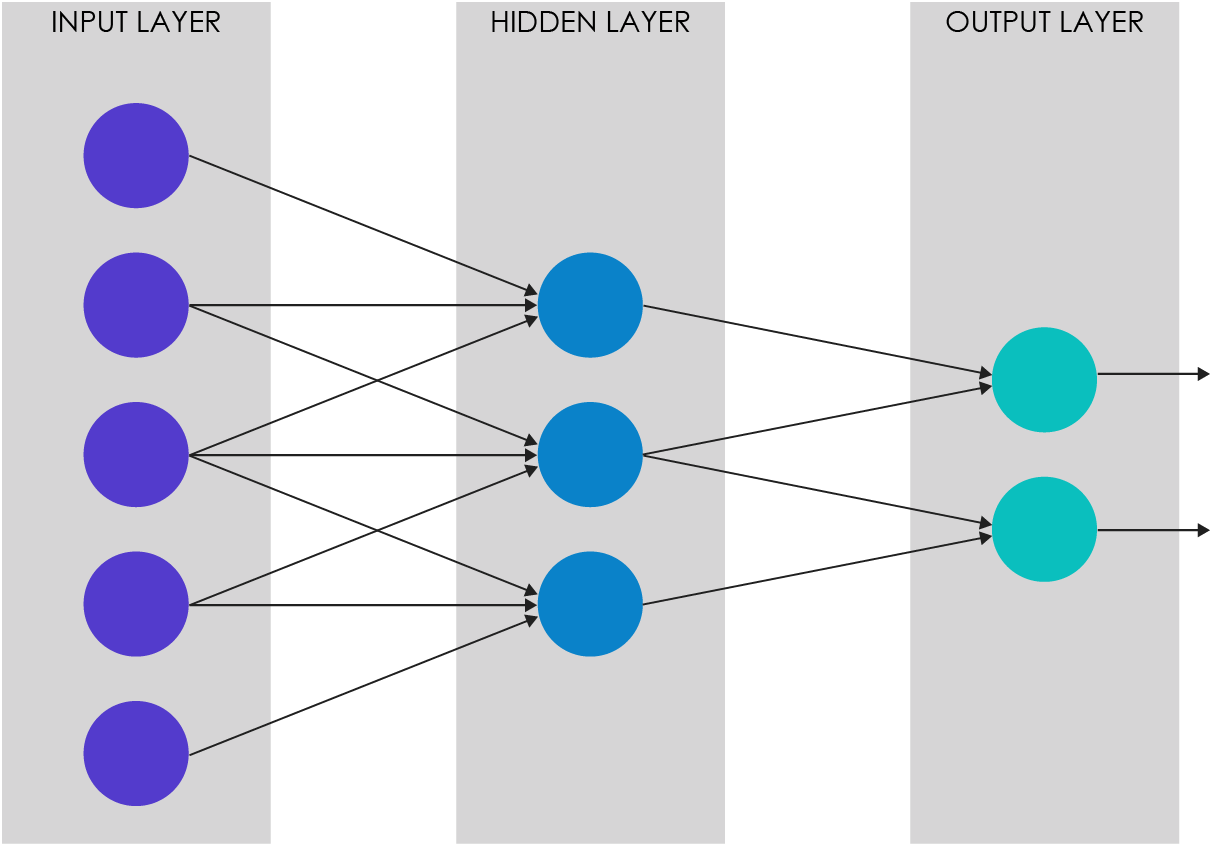
\includegraphics[width=250px]{pictures/cnn.png}
\caption{Convolutional neural network}
\end{figure}

\subsubsection{Recurrent neural network}
In recurrent neural network (RNN) connections between the neurons form a directed cycle. It means that RNN can use its internal memory to learn  sequences of inputs. The same set of weights is applied recursively to the structure.
\par RNN are used for text or speech recognition.
\begin{figure}[H]
\centering
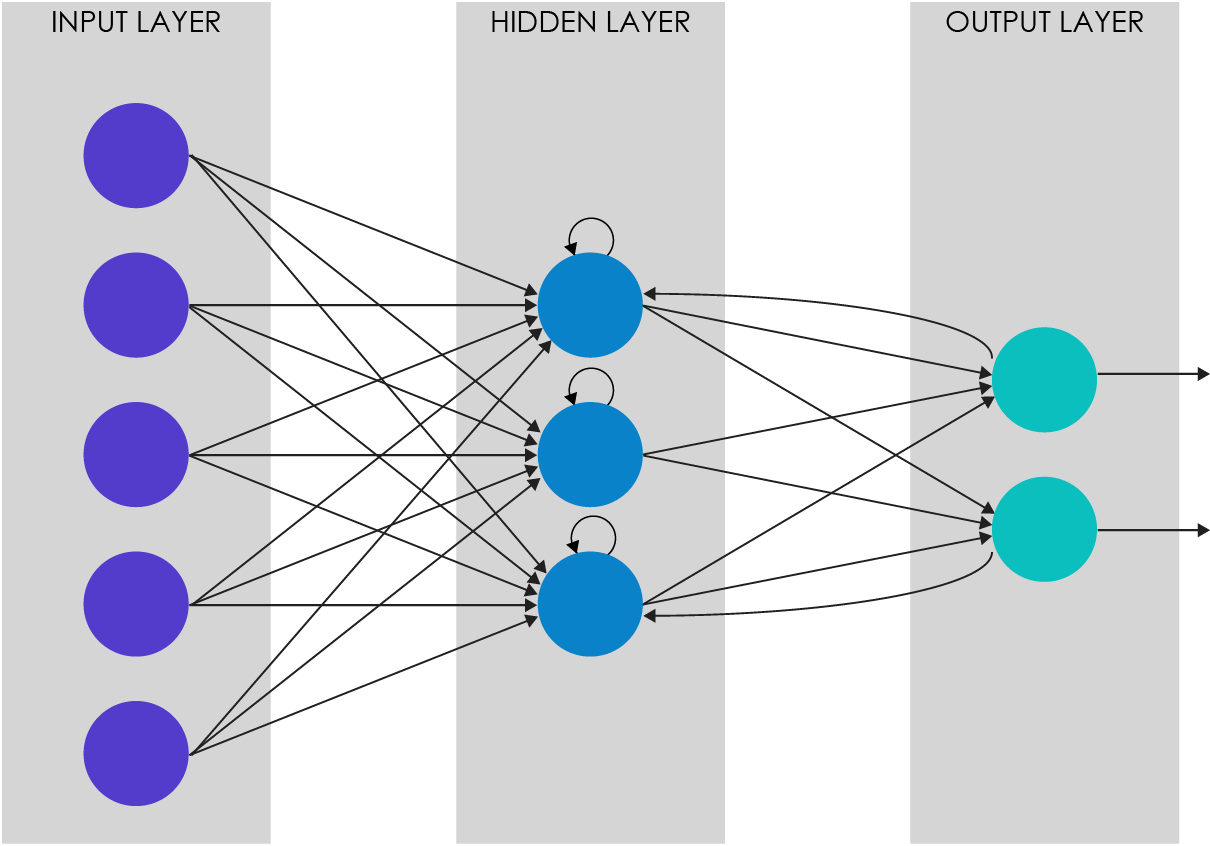
\includegraphics[width=250px]{pictures/rnn.png}
\caption{Convolutional neural network}
\end{figure}

\subsection{Activation function}
The activation function defines the output of considered neuron with given input. There are many functions that can be used as an activation function in artificial neural networks.
\subsubsection{Linear}
\subsubsection{Rectified Linear Unit (ReLU}
\subsubsection{Sigmoid}
\subsubsection{TanH}

\section{Architecture}
\section{Experiments}
\section{Conclusions}
\section{Bibliography}
\end{document}
